%\addcontentsline{toc}{chapter}{Development Process}
\chapter{Design}
\label{section:design}

% \todo[inline]{
% You should concentrate on the more important aspects of the design. It is essential that an overview is presented before going into detail.

% As well as describing the design adopted it must also explain what other designs were considered and why they were rejected.The design should describe what you expected to do, and might also explain areas that you had to revise after some investigation.

% Typically, for an object-oriented design, the discussion will focus on the choice of objects and classes and the allocation of methods to classes. The use made of reusable components should be described and their source referenced. Particularly important decisions concerning data structures usually affect the architecture of a system and so should be described here.How much material you include on detailed design and implementation will depend very much on the nature of the project. It should not be padded out. Think about the significant aspects of your system. For example, describe the design of the user interface if it is a critical aspect of your system, or provide detail about methods and data structures that are not trivial. 

% Do not spend time on long lists of trivial items and repetitive descriptions. If in doubt about what is appropriate, speak to your supervisor. You should also identify any support tools that you used. You should discuss your choice of implementation tools - programming language, compilers, database management system, program development environment, etc. Some example sub-sections may be as follows, but the specific sections are for you to define. 
% }
\section{Hardware}
\begin{figure}
    \centering
    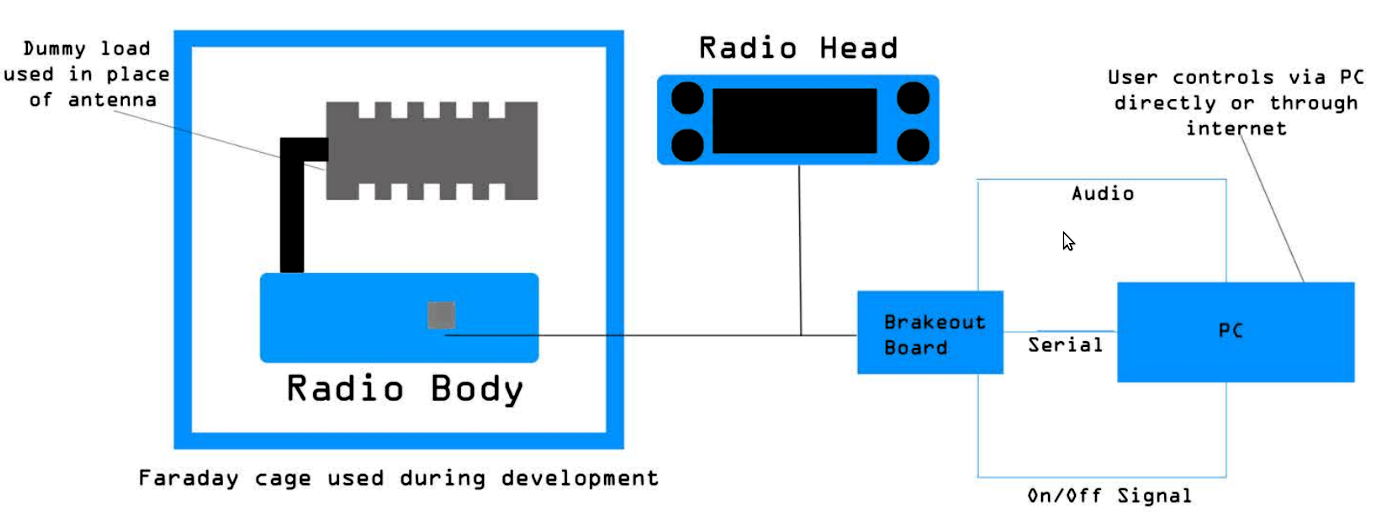
\includegraphics[width=\textwidth]{img/setup_diagram}
    \caption[Hardware Overview]{A hardware overview of the project.}
    \label{fig:setup_diagram}
\end{figure}

\begin{figure}
    \centering
    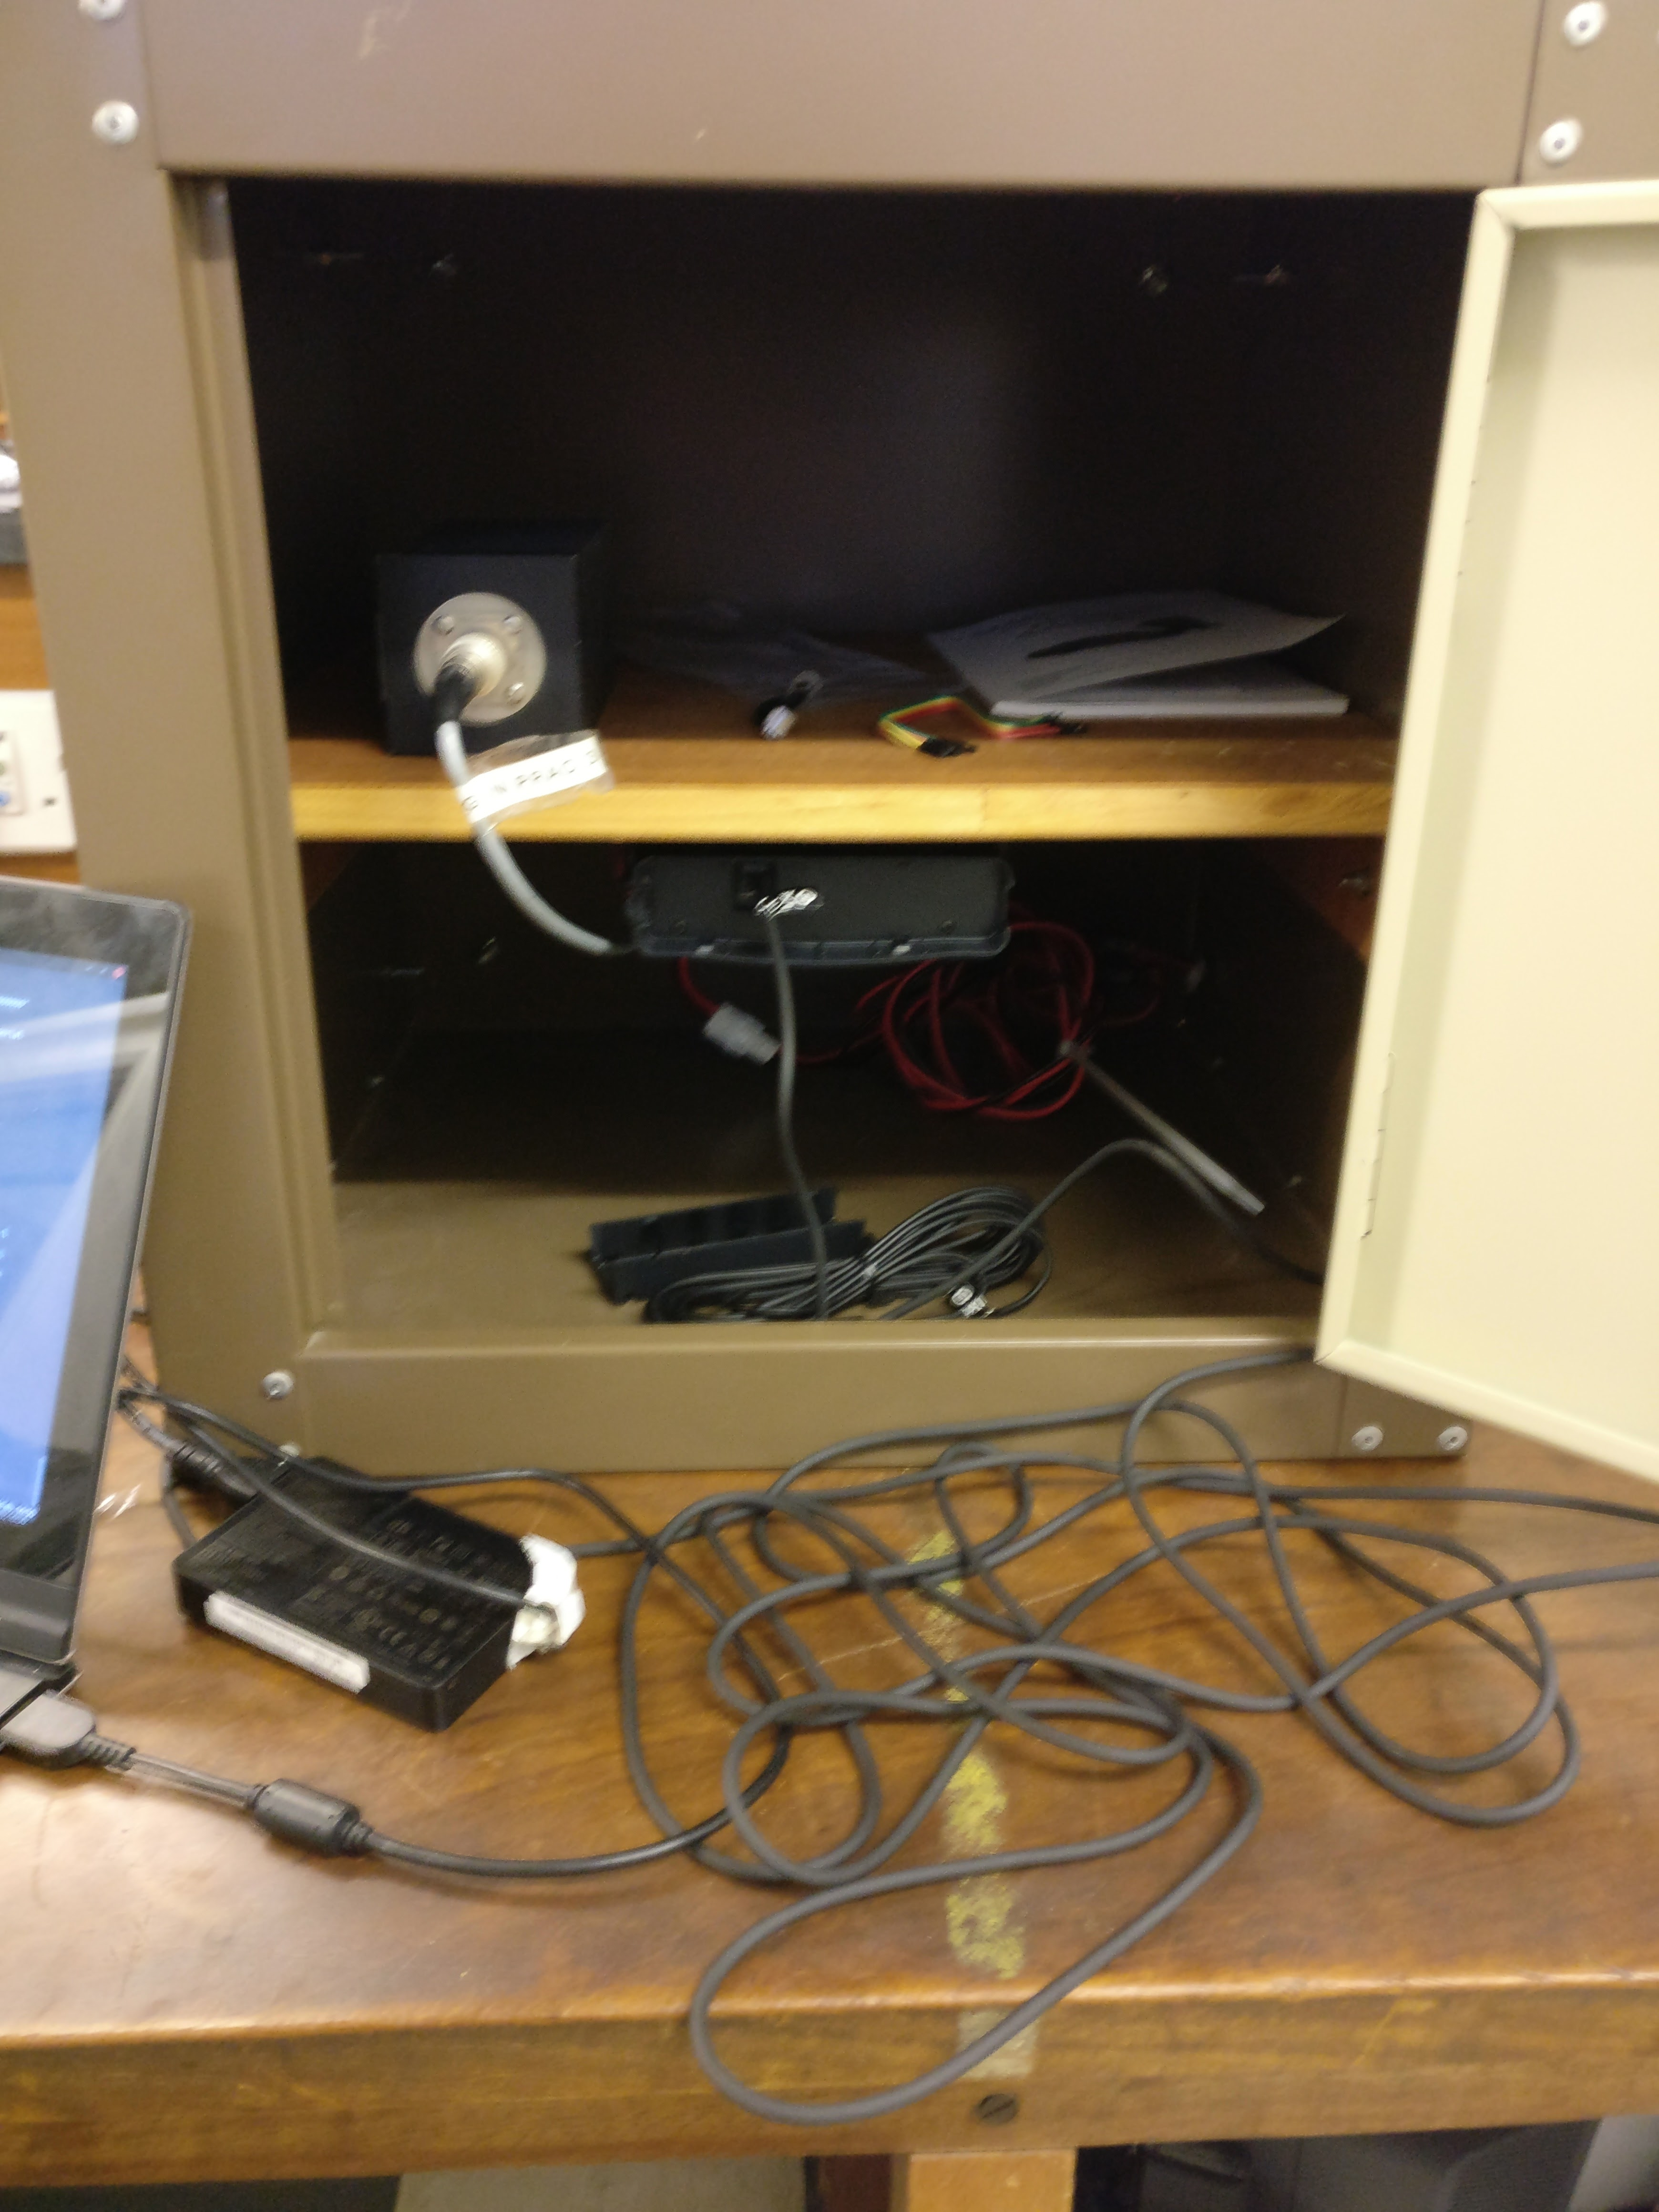
\includegraphics[width=0.5\textwidth]{img/locker.jpg}
    \caption[Radio locker]{A picture of the metal locker used to contain radio waves made from the radio body. The black box below the wooden shelf is the radio body. The box above is the dummy load.}
    \label{fig:locker}
\end{figure}

In order to develop software for the radio, it had to be ensured during development that an error in the program did not lead to rouge transmissions. To do this the radio was suspended on a wooden shelf placed in a grounded metal locker (See Figure~\ref{fig:locker}). Connected to the radio was a dummy load in place of aerial, with power to the radio coming through a whole in the side of the locker so that the door could remain closed. This helped to reduce the strength of any transmissions significantly but not entirely. As a final precaution a second hand-held radio was placed next to the \gls{8900} to monitor for any transmissions. If this was to occur the developer could then shutdown the radio quickly so as to avoid prolonged transmission.

\begin{figure}
    \centering
    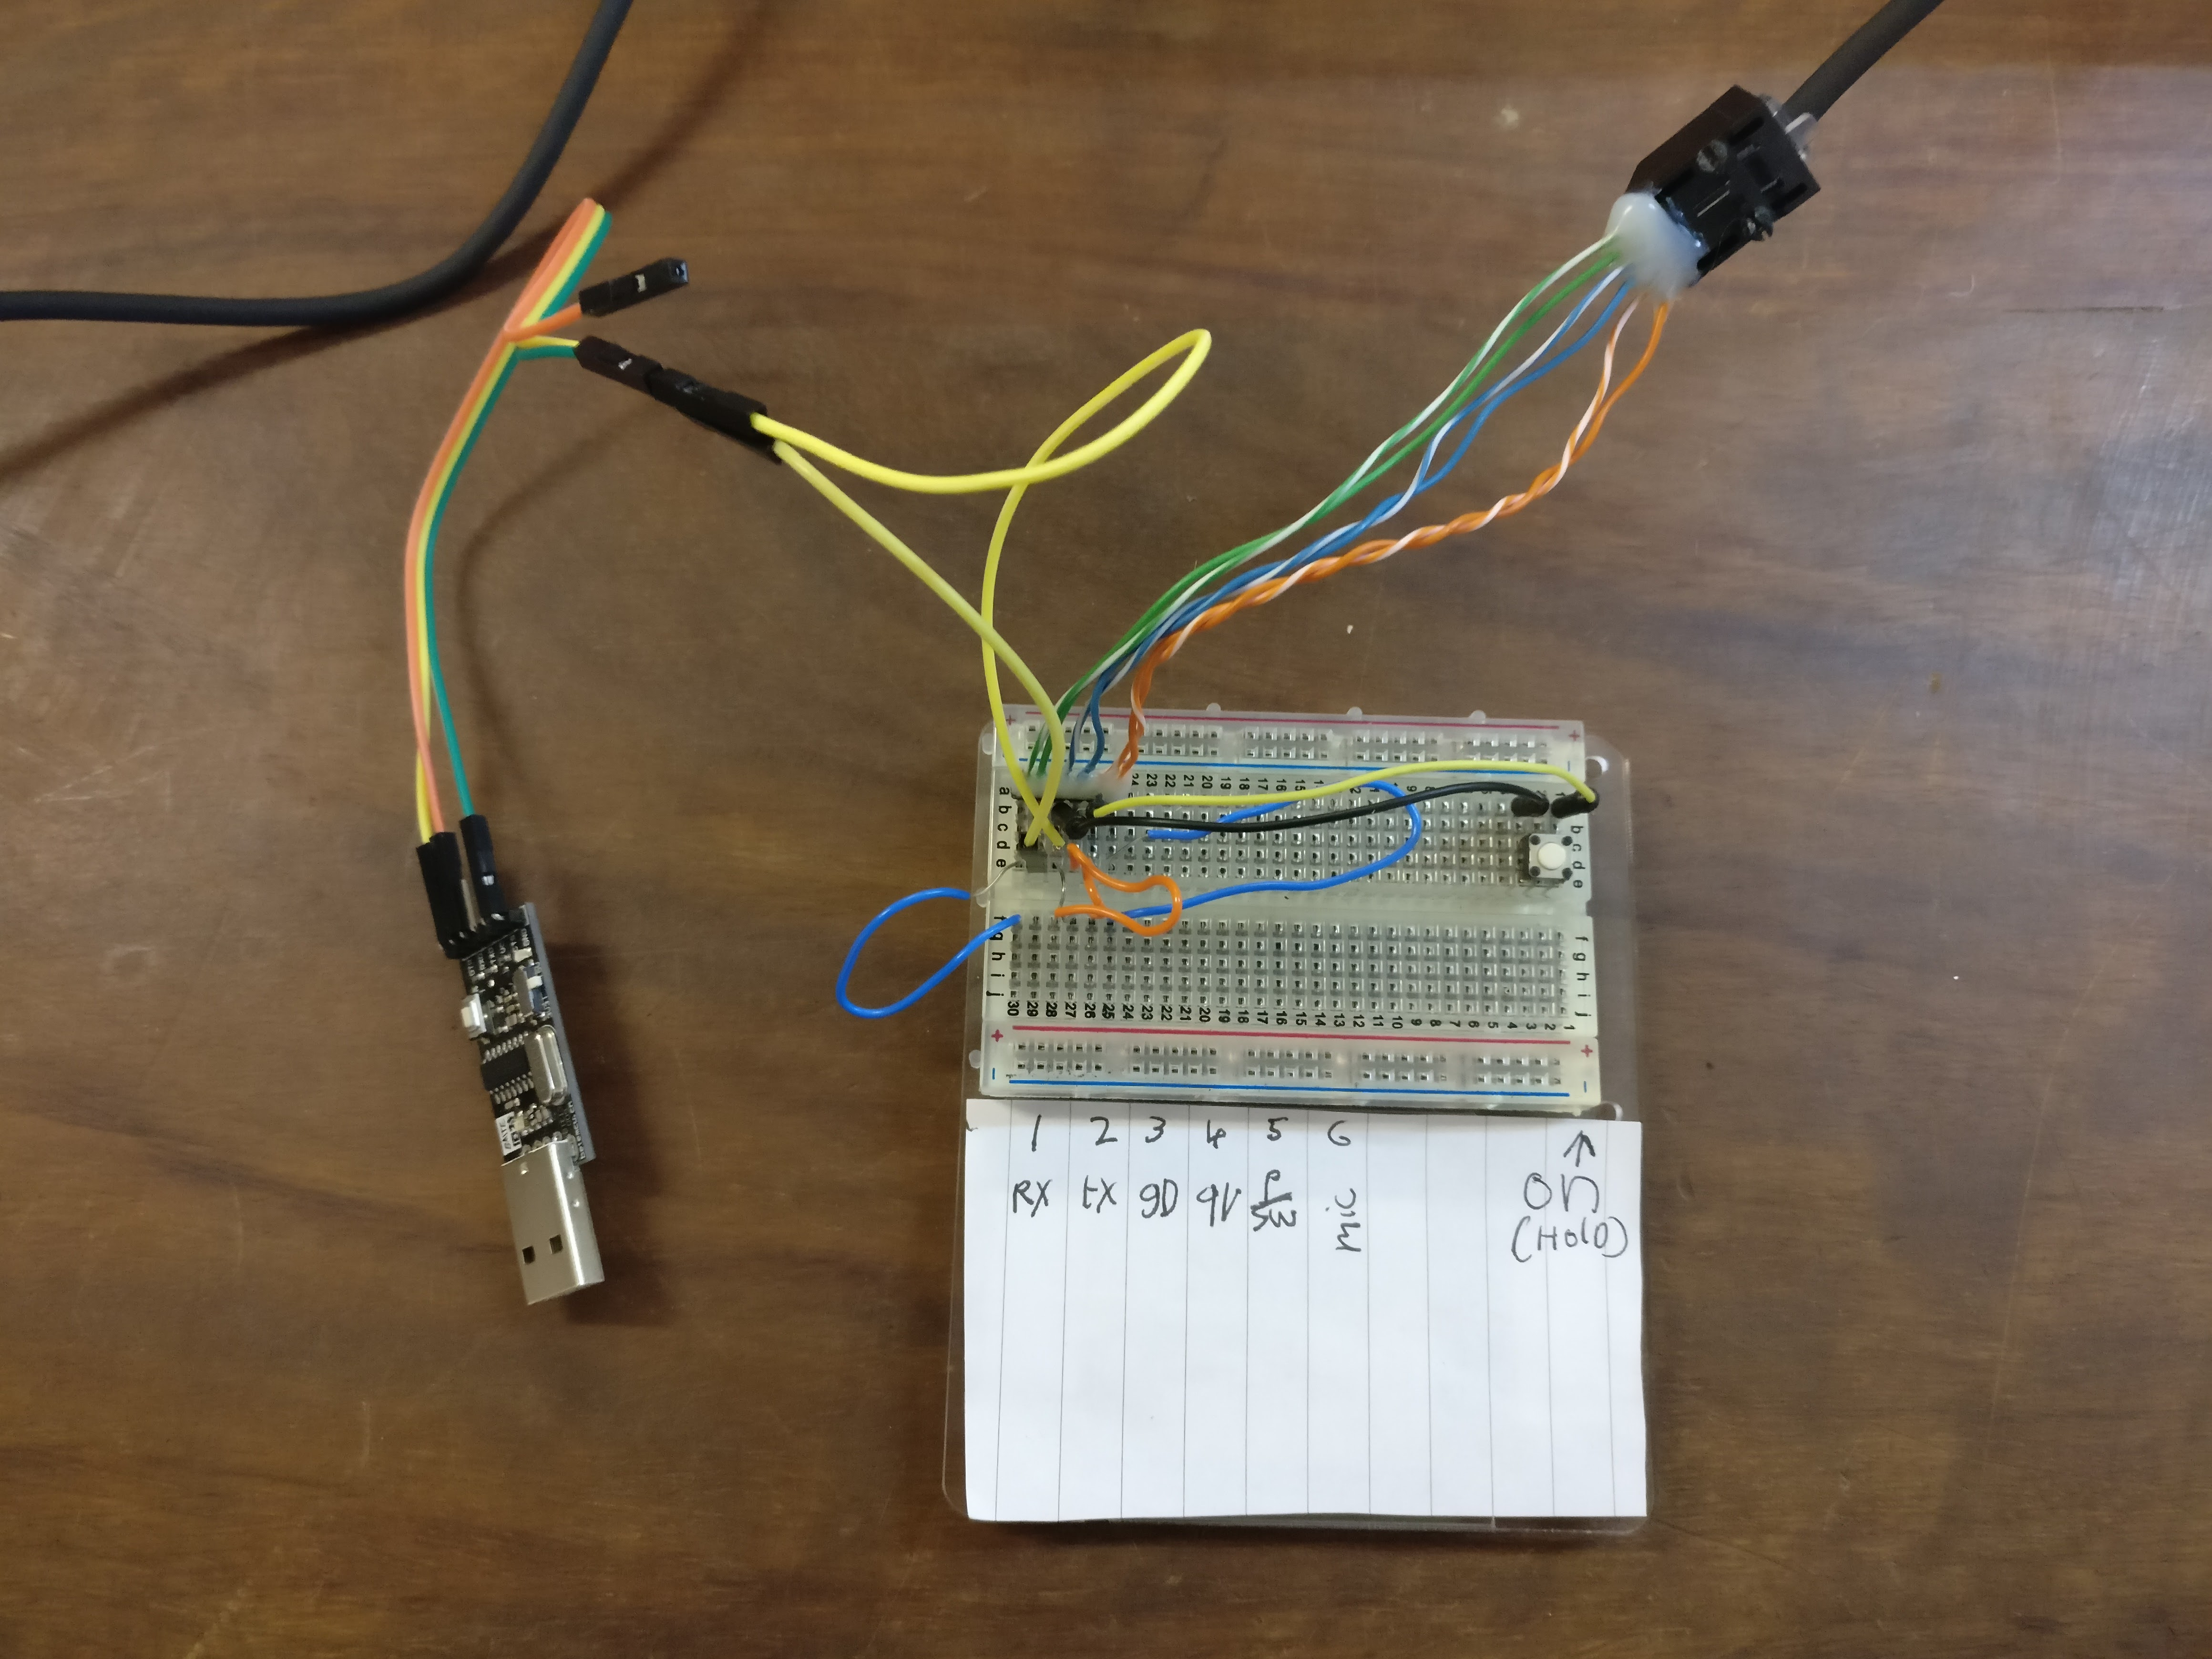
\includegraphics[width=0.9\textwidth]{img/bread_board}
    \caption[Prototype breakout board]{Prototype breakout board used for development.}
    \label{fig:brake_out_board}
\end{figure}

The serial brake-out board (shown in figures~\ref{fig:brake_out_board} and \ref{fig:circuit_diagram}) passes though the required connections to the head of the radio. Allowing the head to still be used, even when the body is controlled by the radio. The ground, \gls{rx} and \gls{tx} serial connections are tapped by the serial dongle with the \gls{tx} being the only disconnected line from the radio. There is also a physical button that connects the power switch to ground when pressed, effectively having the same effect as pressing the power button on the head of the radio.

\begin{figure}
    \centering
    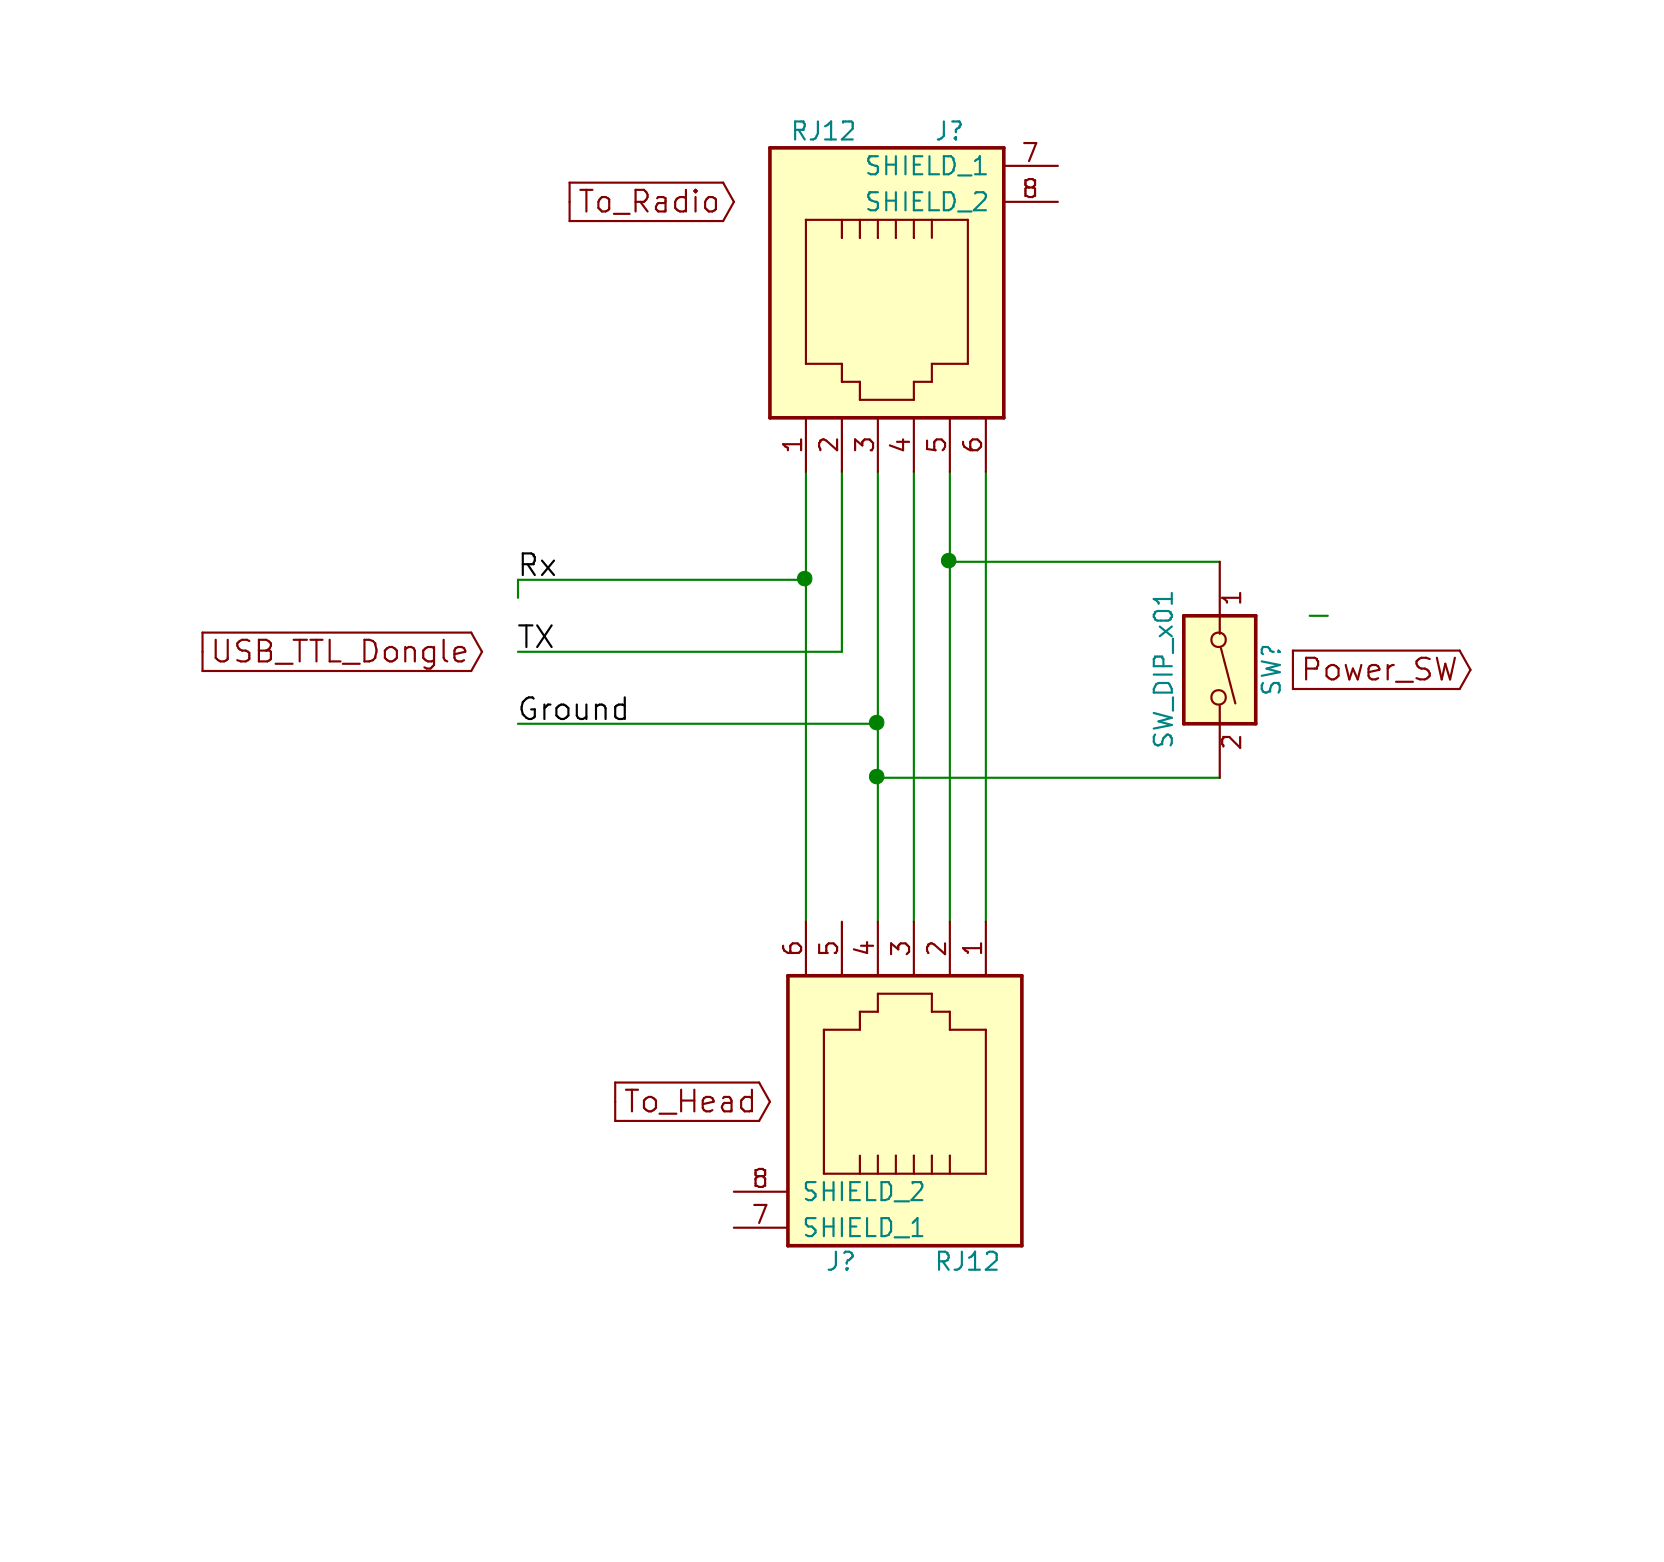
\includegraphics[width=\textwidth]{img/circit.png}
    \caption[Circuit diagram]{Circuit diagram of the brake out board}
    \label{fig:circuit_diagram}
\end{figure}

\section{Overall Architecture}
The more generic functions of the application will be abstracted out to a library so that they can be reused within other applications. The application will provide a console or shell for the user to control the radio from. A console is an appropriate interface as the \gls{xp} methodology demands that designs be made as simple as possible, while still satisfying acceptance tests. Another reason is that the program will ultimately be, an intermediary for signals and not the primary way for the user to control the radio. This is due to the large number of existing and successful free radio control applications designed for such a purpose; for example GRig\cite{grig}. 

\begin{figure}[H]
\centering
    \begin{tikzpicture}[node distance=2cm]
    \node (lib) [process] {libRT8000};
    \node (app) [process, right of=lib, xshift=2cm] {Application};
    \draw [arrow] (lib) -- (app);
    \end{tikzpicture}
    \caption[basic architecture]{The basic overall library/application architecture}
\end{figure}

The the radio must receive packets every 80ms, else it will automatically shutdown. With such a time critical task such as this, the routine was given a separate thread to operate in, so as to lower the impact of other routines on its timing. This is described in figure~\ref{fig:sender_thread}. 

\begin{figure}[ht]
\centering
    \begin{tikzpicture}[node distance=2cm]
% decision, right of=lib, xshift=2cm
    \node (checkq) [decision, xshift=-4cm] {Packet send Queue > 1 ?};
    \node (start) [startstop, above of = checkq, yshift=2cm] {Initialise serial connection, and queue};
        \draw [arrow] (start) -- (checkq);
    
    \node (pop) [process, right of=checkq, xshift=4cm] {Pop and free packet head from memory};
        \draw [arrow] (checkq) -- node[yshift=-0.5cm]{yes}(pop);
        
    \node (peek) [process, below of=pop, yshift=-2cm] {Peek the new head};
        \draw [arrow] (pop) -- (peek);
    
    \node (send) [process, below of=checkq, yshift=-2cm] {Send head packet};
        \draw [arrow] (checkq) -- node[xshift=0.5cm]{No} (send);
        \draw [arrow] (peek) -- (send);
        
    \node (shutdown_q) [decision, left of=send, xshift=-3cm] {Keep alive?};
        \draw [arrow] (send) -- (shutdown_q);
        
    \node (shutdown) [startstop, below of = shutdown_q, yshift=-2cm] {Free remaining queue and return};
        \draw [arrow] (shutdown_q) -- node[xshift=-0.5cm]{No} (shutdown);
        
    \node (wait) [process, left of=checkq, xshift=-3cm] {Sleep 20ms};
        \draw [arrow] (shutdown_q) -- node[xshift=-0.5cm]{Yes} (wait);
        \draw [arrow] (wait) -- (checkq);
    
    \end{tikzpicture}
    \caption[Sender thread]{Flow diagram of the Sender thread}
    \label{fig:sender_thread}
\end{figure}

Items in the queue are only removed (popped) when there is more than a single packet inside. This is done in order to prevent the automatic shutdown of the radio. The effect is that the last packet is kept in the queue and resent continuously until a new packet is added or the program shutdown. 

While designing the packet sender thread the idea of the ``default packet'' was imagined. This packet will contain much of the state of the radio. To change the volume the default packet is directly modified. More complex actions, for example actions that require a button to be pressed only momentarily, will add new packets to the queue. As there will possibly be duplicate packets in the queue, the queue implementation must hold only a reference to the default packet.

It was anticipated that the bulk of memory usage will be to store representations of packets. Therefore the data structure should be as memory efficient as possible. Although this must balance with the ease of use i.e sections being able to be mapped accordingly. Packets are to be stored as a bitfield. This is so that the \gls{rx} packet will take up only 42 bytes (or as close to this as possible). Bit-wise operations would then be used to read and set bits inside the packet. This has the added benefit that sending via serial will not require any additional processing, as the representation is identical.

Packets sent to the screen (\gls{rx}) will hereby be referred to as ``display packets''. These are used to generate the output of the display, where a set bit in the packet corresponds to an illuminated segment on the display. The packets that are \gls{tx} to the radio body will be referred to ``control packets'' as they communicate the current state of the controls back to the radio.

\begin{figure}[H]
\centering
    \begin{tikzpicture}[node distance=2cm]
    \node (app) [process] {Application};
    \node (lib) [process, below of=app] {LibRT8000};
        \draw [arrow] (app) -- (lib);
        \node (control) [process, below of=lib, xshift=-2cm] {Control Packet};
        \node (disp) [process, below of=lib, xshift=2cm] {Display Packet};
        \draw [arrow] (lib) -- (control);
        \draw [arrow] (lib) -- (disp);
            \node (packet) [process, below of=disp, xshift=-2cm] {Packet};
             \draw [arrow] (control) -- (packet);
             \draw [arrow] (disp) -- (packet);
    \end{tikzpicture}
    \caption[Overall architecture]{A more detailed vision of relations of the application}
    \label{overall_architecture}
\end{figure}

\section{Language choice}
\label{section:language_choice}

A number of candidate languages were selected as potentially appropriate. Five main criteria were used to decide what was most appropriate: 
\begin{itemize}
    \item Prior experience
    \item Existing serial support
    \item Ease of bitfield storage
    \item Portability
    \item Speed
\end{itemize}

\section*{Python}
First a scratch program was created to show that it was actually possible to store Bitfields, with mappings to their relevant sections i.e the left volume section (See section \ref{python_bitfield} for this code). This proved promising, but there still remained the question on whether Python could store this in a sufficiently compact manner. In order to test this a 336 bit number (42 bytes) was stored in the interpreter and then queried on how much space had been allocated for it. 

\begin{minted}{python}
>>>import sys

>>>a = (1 << 336)
>>>sys.getsizeof(a)
72
\end{minted}

Python had given a 71\% overhead to the bitfield. 30 bytes more than required is sub-optimal for our usage.

The other concern was how fast the serial library was in Python. While Python does not have serial in its standard library, it does have a well supported third party library named ``PySerial''\cite{pyserial}. A scratch program was written to test this.

\begin{minted}{python}
import serial
ser = serial.Serial('/dev/ttyUSB0')  # open serial port

for _ in range(100):
    ser.write((1 << 336))
    ser.flush() # wait until message sent

ser.close()  
\end{minted}

This program sends 100 x 336 bits as fast as possible to the serial device located named ``ttyUSB0''. The serial line was then connected to a digital oscilloscope in order to measure the performance. The width between packets was a high 40ms, where the actual delay of the radio was 20ms between packets.

At the time this was thought to be unacceptable, however it was later discovered that the body of the radio would take the average of 50ms of received packets before acting and could tolerate up to 80ms of delay before shutting down\cite[pg.21]{ben_report}. However, it was thought that the right choice was made as there was no way to guarantee that these performance issues would not escalate into a larger timing problem further into development. In addition a lower level language would give the application an opportunity to use less system resources.

\section*{Golang}
Golang is a new compiled language created in 2007. It brings many newer ideas that interpreted languages have successfully used such as type inheritance and method overloading. Golang was designed to supplement the C programming language. One of the original authors of Golang is Ken Thompson (who is also one of the original authors of C). Its syntax is a combination of C and python, yet it is more strict than either. For example, including an unused import will induce a compiler error and endorses a definitive style guide instead of multiple competing standards.

Golang could be the ideal language to use in the future, but currently its standard library does not support serial communication. The most supported third party library is still in the alpha stage. This ruled out Golang over competing languages that already had a stable \gls{api} for such actions.

\section*{C}
Other projects of similar nature have used C (including other ham radio drivers). C allows you to define a data structure with a very exact number of bytes.

\begin{minted}[breaklines]{c}
//adapted from http://stackoverflow.com/questions/8584577/access-bits-in-a-char-in-c

//This tells the compiler to not put padding bits between values in the struct.
#pragma pack(1) //as we don't want space between our bits here
typedef struct {
        unsigned int data: 7;      // 7 more bits of the byte
        unsigned int check_num: 1; // Used to signify the first byte in the packet
} FT8900BYTE;

typedef union { 
        FT8900BYTE section;
        unsigned char raw;
} PACKET_BYTE;
#pragma pack()

int main()
{
        PACKET_BYTE packet[42];
        return 0;
}
\end{minted}

C also has serial support in its standard library with the include``<termios.h>''. While this is not as simple to use as other languages, it is the most comprehensive of them by far. Although ``Pyserial'' may have had a had better timeout implementation as it had a hard limit of seconds after the last bit instead of time between packets like the C implementation.

\section*{Comparison}
Table~\ref{table:language_comparison} summarises the comparison of candidate languages. Despite lack of experience, C came out as superior by 11 points. When working in C, a quick check of how much involvement of strings there will be is necessary, as strings are a weakness of the language. Only the logging and shell would involve heavy use of strings, meaning that the bulk of the code would not be affected.

\begin{table}[h!]
\centering
\begin{tabular}{|l| c c c c c |c|} 
 \hline
 Language & experience & serial support & bitfield storage & portability & speed & total\\
 \hline\hline
  Python & 9 & 5 & 5 & 6 & 4 & 29 \\
 \hline
 Golang  & 4 &  2 &  8 &  7 & 10 & 31\\
 \hline
 C       & 2 & 10 & 10 & 10 & 10 & 42\\
\hline
\end{tabular}
\caption{Summary of languages comparison}
\label{table:language_comparison}
\end{table}


